%!TEX root = ../Report.tex 

% This information is used in titlepage, colophon, preface and hyperref setup (pdf metainfo), and other options.

\def\thesistypeabbr{TR}
\def\thesistype    {Technical Report}

\def\thesisauthor  {André Santos, Jean Brito, Luís Costa, João Laranjo, Rui Coelho}
\def\thesistitle   {AMazING}
\def\thesissubtitle{Plataforma de controlo de testes wireless com unidades móveis}
\def\thesislocation{\copyright~Universidade de Aveiro,}

\def\papersize    {a4paper} % Final paper size (b5paper/a4paper), recommended paper size is b5paper
\def\showtrims    {false} % Print on larger paper than \papersize and show trim marks (true/false)?

\def\showtodos    {true}  % Show todos (true/false)?
\def\confidential {false} % Confidential report (true/false)?





%!TEX TS-program = xelatex
%!TEX root = Report.tex
\RequirePackage[l2tabu,orthodox]{nag} % Old habits die hard
 

\newcommand{\papersizeswitch}[3]{\ifnum\strcmp{\papersize}{#1}=0#2\else#3\fi}
\papersizeswitch{b5paper}{\def\classfontsize{10pt}}{\def\classfontsize{12pt}}

\documentclass[openany,\classfontsize,\papersize,twoside,showtrims,extrafontsizes]{memoir}

%!TEX root = ../Report.tex 
% \RequirePackage[l2tabu,orthodox]{nag} % Old habits die hard

% \newcommand{\papersizeswitch}[3]{\ifnum\strcmp{\papersize}{#1}=0#2\else#3\fi}
% \papersizeswitch{b5paper}{\def\classfontsize{10pt}}{\def\classfontsize{12pt}}

% \documentclass[\classfontsize,\papersize,twoside,showtrims,extrafontsizes]{memoir}
\RequireXeTeX

\showtrimsoff
\papersizeswitch{b5paper}{
    % Stock and paper layout
    \pagebv
    \setlrmarginsandblock{26mm}{20mm}{*}
    \setulmarginsandblock{35mm}{30mm}{*}
    \setheadfoot{8mm}{10mm}
    \setlength{\headsep}{7mm}
    \setlength{\marginparwidth}{18mm}
    \setlength{\marginparsep}{2mm}
}{
    \papersizeswitch{a4paper}{
        \pageaiv
        \setlength{\trimtop}{0pt}
        \setlength{\trimedge}{\stockwidth}
        \addtolength{\trimedge}{-\paperwidth}
        \settypeblocksize{634pt}{448.13pt}{*}
        \setulmargins{4cm}{*}{*}
        \setlrmargins{*}{*}{0.66}
        \setmarginnotes{17pt}{51pt}{\onelineskip}
        \setheadfoot{\onelineskip}{2\onelineskip}
        \setheaderspaces{*}{2\onelineskip}{*}
    }{
    }
}
\ifnum\strcmp{\showtrims}{true}=0
    % For printing B5 on A4 with trimmarks
    \showtrimson
    \papersizeswitch{b5paper}{\stockaiv}{\stockaiii}
    \setlength{\trimtop}{\stockheight}
    \addtolength{\trimtop}{-\paperheight}
    \setlength{\trimtop}{0.5\trimtop}
    \setlength{\trimedge}{\stockwidth}
    \addtolength{\trimedge}{-\paperwidth}
    \setlength{\trimedge}{0.5\trimedge}
    
    % bigger todos if trim marks
    \setmarginnotes{10pt}{95pt}{\onelineskip}

    \trimLmarks
    
    % put jobname in left top trim mark
    \renewcommand*{\tmarktl}{%
      \begin{picture}(0,0)
        \unitlength 1mm
        \thinlines
        \put(-2,0){\line(-1,0){18}}
        \put(0,2){\line(0,1){18}}
        \put(3,15){\normalfont\ttfamily\fontsize{8bp}{10bp}\selectfont\jobname\ \
          \today\ \ 
          \printtime\ \ 
          Page \thepage}
      \end{picture}}

    % Remove middle trim marks for cleaner layout
    \renewcommand*{\tmarktm}{}
    \renewcommand*{\tmarkml}{}
    \renewcommand*{\tmarkmr}{}
    \renewcommand*{\tmarkbm}{}
\fi

\checkandfixthelayout                 % Check if errors in paper format!
\sideparmargin{outer}                 % Put sidemargins in outer position (why the fuck is this option not default by the class?)

% Large environments
\usepackage{microtype}
\usepackage{mathtools}
\usepackage{listings}                 % Source code printer for LaTeX
\usepackage{tikz}

% Links
\usepackage[hyphens]{url}             % Allow hyphens in URL's
\usepackage[unicode=false,psdextra]{hyperref}                 % References package

% Graphics and colors
\usepackage{graphicx}                 % Including graphics and using colours
\usepackage{xcolor}                   % Defined more color names
\usepackage{eso-pic}                  % Watermark and other bag
\usepackage{preamble/dtucolors}
\graphicspath{{graphics/}}

% Language
\usepackage{polyglossia}    % multilingual typesetting and appropriate hyphenation
\setdefaultlanguage{english}
\usepackage{csquotes}       % language sensitive quotation facilities

% Bibliography (references)
\usepackage[backend=biber,
            style=alphabetic,
            %backref=true,
            abbreviate=false,
            dateabbrev=false,
            alldates=long]{biblatex}

% Floating objets, captions and references
\usepackage{flafter}  % floats is positioned after or where it is defined! 
%\setfloatlocations{figure}{bhtp}   % Set floats for all figures
%\setfloatlocations{table}{bhtp}    % Set floats for all tables
%\setFloatBlockFor{section}         % Typeset floats before each section
\usepackage[noabbrev,nameinlink,capitalise]{cleveref} % Clever references. Options: "fig. !1!" --> "!Figure 1!"
\hangcaption
\captionnamefont{\bfseries}
\subcaptionlabelfont{\bfseries}
\newsubfloat{figure}
\newsubfloat{table}
%\letcountercounter{figure}{table}         % Consecutive table and figure numbering
%\letcountercounter{lstlisting}{table}     % Consecutive table and listings numbering
\captiontitlefinal{.}
% strip things from equation references, making them "(1)" instead of "Equation~1"
% from http://tex.stackexchange.com/questions/122174/how-to-strip-eq-from-cleveref
\crefformat{equation}{(#2#1#3)}
\crefrangeformat{equation}{(#3#1#4) to~(#5#2#6)}
\crefmultiformat{equation}{(#2#1#3)}%
{ and~(#2#1#3)}{, (#2#1#3)}{ and~(#2#1#3)}

% Table of contents (TOC)
\setcounter{tocdepth}{1}              % Depth of table of content
\setcounter{secnumdepth}{2}           % Depth of section numbering
\setcounter{maxsecnumdepth}{3}        % Max depth of section numbering

% Todos
\usepackage{totcount}                 % For total counting of counters
\def\todoshowing{}
\ifnum\strcmp{\showtodos}{false}=0
    \def\todoshowing{disable}
\fi
\usepackage[colorinlistoftodos,\todoshowing]{todonotes} % Todonotes package for nice todos
\newtotcounter{todocounter}           % Creates counter in todo
\let\oldtodo\todo
\newcommand*{\newtodo}[2][]{\stepcounter{todocounter}\oldtodo[#1]{\thesection~(\thetodocounter)~#2}}
\let\todo\newtodo
\let\oldmissingfigure\missingfigure
\newcommand*{\newmissingfigure}[2][]{\stepcounter{todocounter}\oldmissingfigure[#1]{\thesection~(\thetodocounter)~#2}}
\let\missingfigure\newmissingfigure
\makeatletter
\newcommand*{\mylistoftodos}{% Only show list if there are todos
\if@todonotes@disabled
\else
    \ifnum\totvalue{todocounter}>0
        \markboth{\@todonotes@todolistname}{\@todonotes@todolistname}
        \phantomsection\todototoc
        \listoftodos
    \else
    \fi
\fi
}
\makeatother
\newcommand{\lesstodo}[2][]{\todo[color=green!40,#1]{#2}}
\newcommand{\moretodo}[2][]{\todo[color=red!40,#1]{#2}}

% Chapterstyle
\makeatletter
\makechapterstyle{mychapterstyle}{
    \chapterstyle{default}
    \def\format{\normalfont\sffamily}

    \setlength\beforechapskip{0mm}

    \renewcommand*{\chapnamefont}{\format\HUGE}
    \renewcommand*{\chapnumfont}{\format\fontsize{54}{54}\selectfont}
    \renewcommand*{\chaptitlefont}{\format\fontsize{42}{42}\selectfont}

    \renewcommand*{\printchaptername}{\chapnamefont\MakeUppercase{\@chapapp}}
    \patchcommand{\printchaptername}{\begingroup\color{dtugray}}{\endgroup}
    \renewcommand*{\chapternamenum}{\space\space}
    \patchcommand{\printchapternum}{\begingroup\color{dtured}}{\endgroup}
    \renewcommand*{\printchapternonum}{%
        \vphantom{\printchaptername\chapternamenum\chapnumfont 1}
        \afterchapternum
    }

    \setlength\midchapskip{1ex}

    \renewcommand*{\printchaptertitle}[1]{\raggedleft \chaptitlefont ##1}
    \renewcommand*{\afterchaptertitle}{\vskip0.5\onelineskip \hrule \vskip1.3\onelineskip}
}
\makeatother
\chapterstyle{mychapterstyle}

% Header and footer
\def\hffont{\sffamily\small}
\makepagestyle{myruled}
\makeheadrule{myruled}{\textwidth}{\normalrulethickness}
\makeevenhead{myruled}{\hffont\thepage}{}{\hffont\leftmark}
\makeoddhead{myruled}{\hffont\rightmark}{}{\hffont\thepage}
\makeevenfoot{myruled}{}{}{}
\makeoddfoot{myruled}{}{}{}
\makepsmarks{myruled}{
    \nouppercaseheads
    \createmark{chapter}{both}{shownumber}{}{\space}
    \createmark{section}{right}{shownumber}{}{\space}
    \createplainmark{toc}{both}{\contentsname}
    \createplainmark{lof}{both}{\listfigurename}
    \createplainmark{lot}{both}{\listtablename}
    \createplainmark{bib}{both}{\bibname}
    \createplainmark{index}{both}{\indexname}
    \createplainmark{glossary}{both}{\glossaryname}
}
\pagestyle{myruled}
\copypagestyle{cleared}{myruled}      % When \cleardoublepage, use myruled instead of empty
\makeevenhead{cleared}{\hffont\thepage}{}{} % Remove leftmark on cleared pages

\makeevenfoot{plain}{}{}{}            % No page number on plain even pages (chapter begin)
\makeoddfoot{plain}{}{}{}             % No page number on plain odd pages (chapter begin)

% \*section, \*paragraph font styles
\setsecheadstyle              {\huge\sffamily\raggedright}
\setsubsecheadstyle           {\LARGE\sffamily\raggedright}
\setsubsubsecheadstyle        {\Large\sffamily\raggedright}
%\setparaheadstyle             {\normalsize\sffamily\itseries\raggedright}
%\setsubparaheadstyle          {\normalsize\sffamily\raggedright}


% Hypersetup
\hypersetup{
    pdfauthor={\thesisauthor{}},
    pdftitle={\thesistitle{}},
    pdfsubject={\thesissubtitle{}},
    pdfdisplaydoctitle,
    bookmarksnumbered=true,
    bookmarksopen,
    breaklinks,
    linktoc=all,
    plainpages=false,
    unicode=true,
    colorlinks=false,
    citebordercolor=dtured,           % color of links to bibliography
    filebordercolor=dtured,           % color of file links
    linkbordercolor=dtured,           % color of internal links (change box color with linkbordercolor)
    urlbordercolor=s13,               % color of external links
    hidelinks,                        % Do not show boxes or colored links.
}

\makeatletter
\renewcommand{\@memb@bchap}{%
  \ifnobibintoc\else
    \phantomsection
    \addcontentsline{toc}{chapter}{\bibname}%
  \fi
  \chapter*{\bibname}%
  \bibmark
  \prebibhook
}
\let\oldtableofcontents\tableofcontents
\newcommand{\newtableofcontents}{
    \@ifstar{\oldtableofcontents*}{
        \phantomsection\addcontentsline{toc}{chapter}{\contentsname}\oldtableofcontents*}}
\let\tableofcontents\newtableofcontents
\makeatother

% Confidential
\newcommand{\confidentialbox}[1]{
    \put(0,0){\parbox[b][\paperheight]{\paperwidth}{
        \begin{vplace}
            \centering
            \scalebox{1.3}{
                \begin{tikzpicture}
                    \node[very thick,draw=red!#1,color=red!#1,
                          rounded corners=2pt,inner sep=8pt,rotate=-20]
                          {\sffamily \HUGE \MakeUppercase{Confidential}};
                \end{tikzpicture}
            }
        \end{vplace}
    }}
}

% Prefrontmatter
\newcommand{\prefrontmatter}{
    \pagenumbering{alph}
    \ifnum\strcmp{\confidential}{true}=0
        \AddToShipoutPictureBG{\confidentialbox{10}}   % 10% classified box in background on each page
        \AddToShipoutPictureFG*{\confidentialbox{100}} % 100% classified box in foreground on first page
    \fi
}

% DTU frieze
\newcommand{\frieze}{%
    \AddToShipoutPicture*{
        \put(0,0){
            \parbox[b][\paperheight]{\paperwidth}{%
                
\includegraphics[width=0.5\textwidth]{images/ua.png}
                \vspace*{2.5cm}
            }
        }
    }
}

% This is a double sided book. If there is a last empty page lets use it for some fun e.g. the frieze.
% NB: For a fully functional hack the \clearpage used in \include does some odd thinks with the sequence numbering. Thefore use \input instead of \include at the end of the book. If bibliography is used at last everything should be ok.
\makeatletter
% Adjust so gatherings is allowd for single sheets too! (hacking functions in memoir.dtx)
\patchcmd{\leavespergathering}{\ifnum\@memcnta<\tw@}{\ifnum\@memcnta<\@ne}{
    \leavespergathering{1}
    % Insert the frieze
    \patchcmd{\@memensuresigpages}{\repeat}{\repeat\frieze}{}{}
}{}
\makeatother

%!TEX root = ../Report.tex 

% Text fonts (http://www.macfreek.nl/memory/Fonts_in_LaTeX)
% Install fonts from /usr/local/texlive/<version>/texmf-dist/fonts/opentype/public
\usepackage{fontspec}

% Sans-serif font
\setsansfont[
    Ligatures=TeX,
    Extension=.otf,
    UprightFont=*-regular,
    BoldFont=*-bold,
    ItalicFont=*-italic,
    BoldItalicFont=*-bolditalic,
    Scale=0.8      % Adjustmens when using math in sections
]{texgyreadventor}


%!TEX root = ../Report.tex 

% Content specific packages.

\usepackage{blindtext}
\usepackage{algorithm}
\usepackage{algpseudocode}
%\usepackage{pgfplots}                 % Plot tools
%\usetikzlibrary{
%    arrows,
%    matrix,
%    positioning,
%    shapes,
%    topaths,
%}
%\pgfplotsset{compat=1.7}

% Listings
\lstset{
    basicstyle=\footnotesize\ttfamily,% the size of the fonts that are used for the code
    breakatwhitespace=false,          % sets if automatic breaks should only happen at whitespace
    breaklines=true,                  % sets automatic line breaking
    captionpos=b,                     % sets the caption-position to bottom
    commentstyle=\color{s14a},        % comment style
    deletekeywords={},                % if you want to delete keywords from the given language
    escapeinside={\%*}{*)},           % if you want to add LaTeX within your code
    frame=single,                     % adds a frame around the code
    keywordstyle=\bfseries\ttfamily\color{s09}, % keyword style
    language=Python,                  % the language of the code
    morekeywords={*,...},             % if you want to add more keywords to the set
    numbers=left,                     % where to put the line-numbers; possible values are (none, left, right)
    numbersep=5pt,                    % how far the line-numbers are from the code
    numberstyle=\sffamily\tiny\color{dtugray}, % the style that is used for the line-numbers
    rulecolor=\color{dtugray},        % if not set, the frame-color may be changed on line-breaks within not-black text (e.g. comments (green here))
    showspaces=false,                 % show spaces everywhere adding particular underscores; it overrides 'showstringspaces'
    showstringspaces=false,           % underline spaces within strings only
    showtabs=false,                   % show tabs within strings adding particular underscores
    stepnumber=1,                     % the step between two line-numbers. If it's 1, each line will be numbered
    stringstyle=\color{s07},          % string literal style
    tabsize=2,                        % sets default tab size to 2 spaces
    title=\lstname,                   % show the file name of files included with \lstinputlisting; also try caption instead of title
}

\usepackage{pdflscape}
\usepackage{acronym}
%\usepackage{natbib}
\usepackage{amsmath}
\usepackage{enumitem}
\usepackage{lipsum}  

\addbibresource{bibliography/Bibliography.bib}


\begin{document}
\renewcommand{\chaptername}{Capítulo}
\renewcommand{\listfigurename}{Índice de Imagens}
\renewcommand{\listtablename}{Índice de Tabelas}
\renewcommand{\contentsname}{Índice}
\renewcommand{\appendixname}{Anexo}
\renewcommand{\figurename}{Figura}
\renewcommand{\tablename}{Tabela}

\newcommand{\SubItem}[1]{
    {\setlength\itemindent{15pt} \item[-] #1}
}

\prefrontmatter
%!TEX root = ../Report.tex 
\thispagestyle{empty}             % No page numbers
\calccentering{\unitlength}
\begin{adjustwidth*}{\unitlength}{-\unitlength}
    \begin{adjustwidth}{-0.5cm}{-0.5cm}
        \sffamily
        \begin{flushright}
            \thesistypeabbr{} \\*[0cm]
            \thesistype{}\\
        \end{flushright}
        \vspace*{\fill}
        \noindent
        %\includegraphics[width=0.75\textwidth]{CACHET-logo}\\*[0.5cm]
        \HUGE \thesistitle{}\\*[0.2cm]
        \Huge \thesissubtitle{}\\*[1.2cm]
        \parbox[b]{0.5\linewidth}{%
            \LARGE 
            \thesisauthor{}\\*[1.2cm]
            \Large
            \thesislocation{} \the\year
        }
        \hfill
\includegraphics[scale=0.4]{images/ua.png}
    \end{adjustwidth}
\end{adjustwidth*}
\normalfont
\normalsize

\cleartoevenpage
%!TEX root = ../Report.tex 
\thispagestyle{empty} % No page numbers
%\frieze
\vspace*{\fill}
\sffamily

\Large{
\noindent
\textbf{AMazING}\\
\textbf{Plataforma de controlo de testes wireless com unidades móveis}\\
}

\small
\noindent
\textbf{Projeto em Informática}\\
\textbf{Licenciatura em Engenharia Informática}\\
\textbf{Universidade de Aveiro}\\
\textbf{June 2020}\\
\\
André Santos, NMec 84811\\
cachet@ua.pt\\
Jean Brito, NMec 82783\\
@ua.pt\\
João Laranjo, NMec 91153\\
joao.laranjo@ua.pt\\
Luís Costa, NMec 85044\\
lmcosta98@ua.pt\\
Rui Coelho, NMec 86182\\
ruicoelho@ua.pt
\normalsize
\normalfont
\vspace*{2.5cm}

\clearforchapter


\frontmatter
%!TEX root = ../Report.tex
\chapter{Resumo}
O AMazING  (Advanced Mobile wIreless Network playGround) é uma plataforma de testes que tem como objetivo a capacidade de agendar e executar experiências de networking. A rede AMazING é composta por 24 nós fixos com capacidades wireless e um nó móvel (denominado de robô). \newline
Através desta plataforma, de uma forma simples e intuitiva, podemos realizar experiências que podem variar entre o teste de novos protocolos a testes de interferência em redes wireless. Adicionalmente o robô, que possui um nó, está posicionado num carril o que o permite simular os movimentos de um utilizador à medida que se  movimenta em relação aos 24 nós fixos. \newline
Com principal objetivo deste projeto foi estabelecido que este seria o desenvolvimento de uma interface que facilite a interação com os nós acima mencionados e que permita, também, aos utilizadores fazer o agendamento e gestão das suas experiências na plataforma, bem como analisar e visualizar os resultados obtidos em cada uma das suas experiências. É importante realçar que o trabalho a ser realizado com o robô ficou, após diálogo com os orientadores, para segundo plano. Isto devido a uma reestruturação eletrónica no âmbito de trabalhos a ser desenvolvidos em paralelo. Tais motivos tornaram o robô indisponível na realização deste projeto.
Neste documento é apresentado o estudo efetuado relativamente a esta plataforma de testes bem como o seu processo de implementação. De seguida, é descrita a implementação da plataforma, a sua arquitetura e o seu modelo de dados.


\chapter{Palavras-Chave}
\begin{acronym}[Keys]
\acro{Experiência}{Testes realizados sobre os nós existentes na rede}
\acro{APU: Advanced Processing Unit}{Hardware similar a um router utilizado para realizar as experiências de rede}
\acro{SBC: Single Board Computer}{Computador construído numa única placa de circuitos. Possui elementos como um microprocessador(es), memória e I/O. }
\acro{Nó}{APU configurada}
\end{acronym}

\chapter{Agradecimentos}
Gostaríamos de agradecer aos supervisores de projeto, o Professor Flávio Meneses e ao Professor Daniel Corujo pela disponibilidade que demonstraram desde o primeiro momento para nos  ajudar a chegar aos objetivos estabelecidos e a clarificar dúvidas que foram surgindo ao longo das várias fases do projeto.

\clearforchapter
\tableofcontents
\clearforchapter
\listoffigures
\clearforchapter
\listoftables

\mainmatter
%!TEX root = ../Report.tex
\chapter{Introdução}
\label{chp:introduction}
O desenvolvimento de plataformas que facilitem as operações de utilizadores de um dado sistema não é um conceito novo.  A plataforma desenvolvida no decorrer deste projeto tem como público alvo utilizadores com experiência na área de redes e telecomunicações. \newline
Embora o contexto em que este projeto se insere seja bastante específico, é possível encontrar plataformas semelhantes à desenvolvida neste projeto. No entanto, a grande maioria das soluções encontradas são específicas à infraestrutura sobre a qual assentam e as restantes são demasiado generalistas, não considerando todos os detalhes necessários à realização de experiências sobre redes. \newline
Deste modo, tornou-se necessário o desenvolvimento de uma plataforma capaz de responder às necessidades destes utilizadores, surgindo assim o AMazING.

\section{Contexto}
Este projeto foi desenvolvido no âmbito da unidade curricular de Projeto em Informática, inserido na Licenciatura em Engenharia Informática (LEI) da Universidade de Aveiro (UA). O foco do projeto é criação de uma interface que permita fazer o agendamento e gestão de experiências na plataforma de testes, sendo possível consultar os resultados após o término das mesmas. O presente trabalho foi desenvolvido durante o segundo semestre do ano letivo de 2019/2020.

\section{Motivação}
A plataforma AMazING constitui uma mais valia para qualquer pessoa que pretenda realizar testes sobre redes móveis dado que esta permite simular situações reais.\newline
A motivação para este projeto é o desenvolvimento de uma plataforma que ajude essas mesmas pessoas a agendar e gerir as suas experiências e a obter os dados resultantes das mesmas, desse modo, facilitando todo o processo através de um GUI que lhes fornece tudo o que necessitam de forma fácil e intuitiva.

\section{Objetivos}
Este projeto teve como principal objetivo desenvolver uma plataforma intuitiva e de fácil utilização que permita aos seus utilizadores realizar as suas experiências com um nível menor de esforço no que toca à preparação  e  visualização destas.\newline
Após uma reunião com os orientadores do projeto procedeu-se à definição de uma lista de objetivos na qual o desenvolvimento deste projeto se focou. Os objetivos definidos podem ser enunciados da seguinte forma:
\begin{itemize}
    \item Criação de uma plataforma web que agrega todo o trabalho já existente;
    \item Tornar a plataforma intuitiva e fácil de usar como foi mencionado anteriormente;
    \item Tornar a plataforma de testes reconfigurável de modo a que esta se adapte às necessidades de cada utilizador.
    \item Desenvolvimento de uma ferramenta que permite a visualização de informação de cada nó existente na infraestrutura bem como recolher estatísticas e informações importantes numa dada experiência;
    \item A plataforma deve ser capaz de gerir ambientes de diferentes tipos de testes.
\end{itemize}

\section{Impactos do Covid-19}
Durante o desenvolvimento deste projeto houve a clara interferência causada pela situação do Covid-19 e como tal nós reunimos e delineamos não só os impactos mas também as soluções de modo a melhor nos prevenirmos e de modo a que o desenvolvimento não fosse afetado.
Deste modo consideramos que os maiores impactos seriam:
\begin{itemize}
    \item A não existência de reuniões presenciais o que dificulta a comunicação e interação do grupo;
    \item A impossibilidade de reuniões presenciais com os nosso orientadores, tornando todo o processo de transmissão de informação e esclarecimento de dúvidas mais complicado;
    \item A impossibilidade de aceder fisicamente ao IT o que impede as experiências com os equipamento lá presentes, nomeadamente o Switch onde estão conectados os nós, assim como acesso à rede privada de testes;
    \item Devido à impossibilidade de acesso à rede privada de testes foram disponibilizadas 5 APUs para nos possibilitar o avanço do trabalho sem a necessidade de deslocamento ao IT. Seria um para cada membro do grupo no entanto com a divisão de tarefas apenas dois membros do grupo ficaram com APUs - 3 e 2 para os 2 membros encarregues desta parte do projeto;
    \item Impacto da moral e motivação da equipa uma vez que não era possível reunirmo-nos presencialmente e ver os resultados da solução tão claramente.
\end{itemize}

Dado os impactos acima referidos, e após alguma deliberação, foram implementadas as seguintes soluções:
\begin{itemize}
    \item Reuniões semanais presenciais foram substituídas por videoconferências de modo a manter o contacto com os orientadores mais “real”;
    \item O contacto com os orientadores foi feito através de videoconferências e também através canal de slack mais ativo. Em alternativa, caso estes meios não estivessem a funcionar/disponíveis, o contacto foi mantido com a troca de emails;
    \item Os equipamentos foram enviados por correio e apenas quando absolutamente necessário foi feito um deslocamento com as devidas precauções para entrega e troca de algum material;
    \item Utilização de um switch comercial, de modo a substituir o switch Aruba apenas disponível no IT.

\end{itemize}

\subsection{Estrutura do Documento}
O restante documento possui uma estrutura dividida por cinco capítulos. O \textbf{capítulo 2} apresenta uma índole mais analítica, no qual são apresentados os trabalhos existentes nesta área identificando, assim, bases que poderão ser utilizadas para o presente projeto. São, ainda, discutidas as tecnologias que foram utilizadas bem como a explicação da sua utilização no âmbito do projeto. No \textbf{capítulo 3} é realizada uma análise e discussão da arquitetura do sistema bem como dos requisitos fundamentais para o seu bom funcionamento. No \textbf{capítulo 4} é realizada uma análise detalhada da implementação da plataforma abordando os vários pontos, isto é, explicação do frontend, da API de ligação entre o Frontend e a base de dados bem como a comunicação com os APUs e, por fim, a discussão da implementação do módulo de comunicação dos APUs (API Rest). Finalmente, no \textbf{capítulo 5} são enunciadas as conclusões tiradas do projeto bem como toda a aprendizagem associada ao mesmo, apontando ainda possível trabalho futuro que o grupo pensa fazer sentido no contexto do projeto.
%!TEX root = ../Report.tex
\chapter{State of the Art}
Como o nosso projeto aborda um tema não muito comum não é de admirar que não hajam muitas plataformas com o mesmo propósito mas apesar disso ainda há 2 projetos que merecem uma menção.
\section{Projetos relacionados}
No que toca a projetos relacionados achamos que estes 2 merecem uma menção sendo que um é o trabalho previamente efetuado na UA por outro grupo e o outro foi um trabalho publicado por estudantes e investigadores do NICTA (National Information and Communications Technology Australia) e da Universidade Rutgers.
\subsection{NICTA}
Este estudo/trabalho como mencionado acima foi publicado por estudantes e investigadores do NICTA (National Information and Communications Technology Australia) e da Universidade Rutgers e tem como titulo “OMF: A Control and Management Framework for Networking Testbeds” e procura resolver os mesmos problemas que nós pretendemos resolver.
\subsection{PEI 2019}
Este foi o trabalho efetuado previamente na UA por outro grupo de estudantes relativamente a este tópico e foi daqui que adaptamos o nosso projeto, o trabalho realizado por eles está disponível no github porém os focos dos dois projetos divergem ligeiramente.
\section{Tecnologias Utilizadas}
Nesta secção apresentamos de forma sucinta as várias tecnologias que foram utilizadas no desenvolvimento do sistema.
\subsection{PostegreSQL}
PostgresSQL é um sistema open-source de gestão de bases de dados relacionais (Relational Database Management System, RDBMS) coordenado pelo PostgreSQL Global Development Group. A sua criação teve como objetivo manter uma ferramenta open-source, mas com a mesma fidelidade do MySQL.\newline
A estrutura funciona tendo como base tabelas que, por sua vez, têm atributos e utiliza Structured Query Language (SQL) para poder manipular os dados nas mesmas.
Esta tecnologia no contexto deste projeto foi utilizada, essencialmente, para a manutenção de todas as informações associadas à plataforma, isto é, informações sobre as experiências, utilizadores, endereçamento e informações sobre os nós.
\subsection{SQLite}
SQLite é uma biblioteca em linguagem C que implementa um banco de dados SQL embutido. Programas que usam a biblioteca SQLite podem ter acesso a banco de dados SQL sem executar um processo SGBD separado. A biblioteca SQLite lê e escreve diretamente no ficheiro de banco de dados no disco.\newline
A estrutura funciona tendo como base tabelas utilizando a linguagem SQL, tal como a Base de Dados PostgreSQL.\newline
No caso do backend a utilização desta ferramenta teve em vista a testagem das features desenvolvida uma vez que, devido ao covid, o desenvolvimento do projeto foi afetado, foi necessário arranjarmos formas de armazenar informações de testes sem que fosse necessário configurar ambientes de desenvolvimento tão pesados e que pudessem ser facilmente replicados no computador de quem possui os nós, uma vez que os SQLite é um ficheiro de texto, bastava ao membro ter esse ficheiro sem que fossem necessárias configurações extra evitando, assim, de cada vez que fosse necessário mudar tabelas de base de dados tivesse que existir um nosso processo de deployment das mesmas.\newline
No caso do Frontend esta ferramenta foi essencialmente usada para a gestão de logs por parte do administrador do sistema.
%!TEX root = ../Report.tex
\chapter{Requisitos e Arquitetura do Sistema}
\label{chp:requirements}
\section{Requisitos do Sistema}
Esta secção apresenta as especificações gerais dos requisitos do sistema. As seguintes subseções descrevem, em primeiro lugar, o processo de levantamento de requisitos e de seguida o contexto, os atores e os respetivos casos de uso. Por fim, são especificados os requisitos não funcionais do sistema, bem como as dependências do sistema e suposições.

\subsection{Levantamento de requisitos}
O levantamento de requisitos foi realizado na primeira fase de desenvolvimento do projeto,  na fase inicial de desenvolvimento. Foi realizada uma reunião com os Professore Flávio Meneses e o Professor Daniel Corujo na qual foram expostos os principais objetivos da plataforma.\newline
Desse modo, foram tomadas as seguintes decisões:
\begin{itemize}[noitemsep]
    \item Uma plataforma web será o foco principal do projeto sendo que a possibilidade de trabalhar com o nó móvel (também denominado de robô) foi movida para trabalho futuro devido ao facto do mesmo estar a ser alvo de reestruturações mecânicas e eletrónicas;
    \item A utilização da plataforma está restrita para utilizadores autenticados.
        \SubItem{Numa primeira fase serão criados, por um administrador do sistema, utilizadores próprios da plataforma (com um sistema de login com utilizador e palavra passe);}
        \SubItem{Numa fase posterior perspectiva-se a integração com as credenciais de colaboradores do IT através do LDAP.}
    \item Permitir a reconfiguração da rede de nós através da plataforma assim como a visualização dos dados de cada nó e os resultados das variadas experiências;
\end{itemize}

\subsection{Contexto}
Redes sem fios e, mais em particular redes móveis, têm sido um assunto bastante discutido nos dias que correm. Trabalhos de investigação e de inovação têm-se deparado com dificuldades na realização de testes ou experiências em ambiente real. Tal pode acontecer devido ao preço do material, condições ambientais ou difícil reprodução das condições ou ambientes sem fios. Para solucionar este problema surge a plataforma AMazING, uma plataforma de testes wireless com uma interface apelativa e fácil de utilizar.\newline
A plataforma foi desenvolvida de modo a facilitar a configuração dos nós necessários para cada experiência. O utilizador poderá agendar e realizar a sua experiência num ambiente o mais real possível.\newline
É importante referir que, a execução de vários testes em simultâneo seria possível desde que fossem utilizados nós distintos ou fosse garantido o isolamento, através de SDN, no switch. No entanto, devido à complexidade e aos conhecimentos de redes necessários para o desenvolvimento desta feature, foi considerado impossível a implementação da mesma no tempo disponível para a realização do projeto.\newline
Por este motivo, sempre que um utilizador pretenda agendar uma experiência, todos os nós ficam reservados para ele durante um determinado espaço de tempo. 
No menu principal está disposta a grelha de nós e as várias operações possíveis estão divididas em secções na barra de navegação, sendo que cada secção pode ter subsecções que permitem realizar funcionalidades mais específicas.


\subsection{Atores}
A desenvolvimento da interface gráfica foi levado a cabo tendo em conta que a plataforma será utilizada por pessoas que à partida são experientes na sua área, porém mantendo a interface simples de modo a ser de uso fácil. De seguida, enumeramos uma classificação dos atores que irão utilizar a plataforma:
\begin{itemize}
    \item \textbf{Utilizador - Begginer}  – O João é estudante de Mestrado e está a realizar a sua tese no Instituto de Telecomunicações. Encontra-se num projeto de investigação que envolve testes de comunicação (com e sem fios) e desenvolvimento de novos protocolos de redes.\newline 
    O João precisa de realizar os seus testes num ambiente o mais real possível evitando simuladores virtuais. \newline
    O João é um utilizador iniciante, (nível 1) e só lhe é permitido utilizar os templates ao utilizar o sistema. e carregar ficheiros de execução para as APUs.
    \item \textbf{Utilizador - Advanced}  - O João recebe acesso de utilizador avançado (nível 2) o que lhe permite ter acesso direto ao terminal das APUs durante a realização de sua experiência. Podendo assim realizar a instalação de drivers, implementação de protocolos e outros serviços necessários para a realização da experiência
    \item \textbf{Administrador} - O Manuel é professor e Doutorado em Redes e Telecomunicações. É um dos responsáveis pelo Instituto de Telecomunicações e tem experiência em vários projetos relacionados com o desenvolvimento e implementação de novos protocolos de redes e telecomunicações.\newline
    O Manuel precisa de garantir o funcionamento e o acesso aos recursos disponibilizados no IT. 
\end{itemize}

\subsection{Casos de Uso}
Nas imagens seguintes, apresentamos os modelos de casos de uso(CaU) da solução. 
\subsubsection{Utilizador/Tester}
\begin{figure}[!ht]
    \centering
    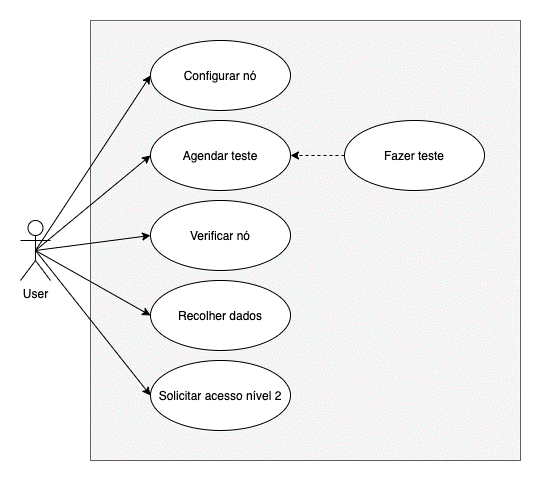
\includegraphics[height=0.36\textheight]{images/CaU1.png}
    \caption{Casos de uso do utilizador/Tester}
    \label{fig:cau1}
\end{figure}
Os casos de usos consoante a sua prioridade podem sintetizados de acordo com a seguinte tabela:
\begin{table}[ht]
    \centering
        \begin{tabular}{p{.25\textwidth}p{.50\textwidth}p{.15\textwidth}}
            \hline
            \textbf{CaU} &	\textbf{Descrição} &	\textbf{Prioridade} \\ 
            \hline
            Configurar Nó & Permite ao utilizador configurar um dado nó da rede como preferir. & Alta \\
            \hline
            Agendar/Fazer teste & Permite ao utilizador agendar a sua experiência e consequentemente efetuá-la no seu tempo alocado. & Alta \\
            \hline
            Verificar nó & Permite ao utilizador ver a informação de um nó (o seu estado, configuração, etc) & Alta \\
            \hline
            Recolher Dados & Permite ao utilizador recolher os dados provenientes da sua experiência. & Alta \\
            \hline
            Solicitar acesso de nível 2 & Permite que utilizador solicite a um administrador uma elevação dos seus privilégios na plataforma. & Alta \\
            \hline
        \end{tabular}
    \caption{Casos de uso do utilizador/Tester}
    \label{myTable}
\end{table}

\subsubsection{Administrador}
\begin{figure}[!ht]
    \centering
    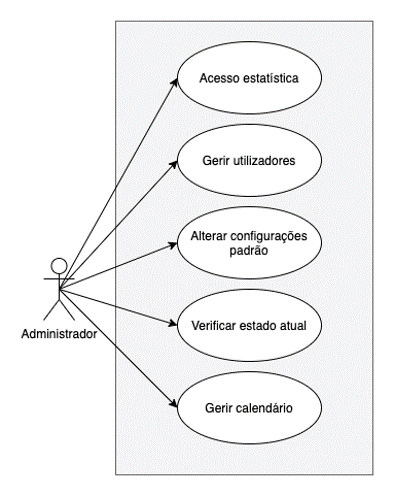
\includegraphics[height=0.4\textheight]{images/CaU2.png}
    \caption{Casos de uso do Administrador}
    \label{fig:cau2}
\end{figure}
Os casos de usos consoante a sua prioridade podem sintetizados de acordo com a seguinte tabela:
\begin{table}[ht]
    \centering
        \begin{tabular}{p{.25\textwidth}p{.50\textwidth}p{.15\textwidth}}
            \hline
            \textbf{CaU} &	\textbf{Descrição} &	\textbf{Prioridade} \\ 
            \hline
            Acesso a estatísticas & Permite ao administrador aceder às estatísticas da plataforma. & Alta \\
            \hline
            Gerir Utilizadores & Permite ao administrador gerir os utilizadores da plataforma assim como elevar o seu nível. & Alta \\
            \hline
            Adicionar/alterar Configurações padrões & Permite ao administrador adicionar/alterar configurações padrão dos nós & Alta \\
            \hline
            Verificar estado atual & Permite ao administrador verificar o estado atual da rede AMazING e dos seus nós. & Alta \\
            \hline
            Gerir Calendário & Permite ao administrador ver e gerir o calendário e os testes agendados. & Alta \\
            \hline
        \end{tabular}
    \caption{Casos de uso do Administrador}
    \label{myTable}
\end{table}

\newpage

\subsection{Requisitos não funcionais}
Abaixo, apresentamos os requisitos não funcionais do sistema.
\begin{itemize}
    \item \textbf{Usabilidade: } dado o principal propósito da aplicação, é necessário que esta seja simples de aprender e utilizar;
    \item \textbf{Autenticação:} A utilização da aplicação deve ser disponível apenas para utilizadores do IT 
        \SubItem{Numa primeira fase, adicionados ao sistema por um administrador;}
        \SubItem{Numa segunda fase, possuindo autenticação pelas credenciais de colaboradores do IT através do LDAP.}
    \item \textbf{Controlo:} O administrador do sistema deve ser capaz de configurar e realizar a manutenção do sistema;
    \item \textbf{Dados:} Os utilizadores do sistema deve conseguir aceder aos dados da experiência realizada.

\end{itemize}

\subsubsection{Suposições e Dependências}
Para o funcionamento completo do sistema, é necessário que sejam configurados os seguintes:
\begin{table}[ht]
    \centering
        \begin{tabular}{|p{.30\textwidth}|p{.60\textwidth}|}
            \hline
            \textbf{Hardware} &	\textbf{Software}\\ 
            \hline
            \begin{itemize}
                \item APUs
                \item Switch Aruba
            \end{itemize}
            & 
            \begin{itemize}
                \item Base de Dados Relacional de linguagem SQL
                \item Flask
                    \SubItem{No servidor principal}
                    \SubItem{Em cada uma das APUs}
                \item Django + SQLite
                \item Web SSH server
            \end{itemize}
            \\
        \hline
        \end{tabular}
    \caption{Componentes necessárias para o funcionamento}
    \label{myTable}
\end{table}

\section{Arquitetura do sistema}
Esta secção apresenta uma vista geral da arquitetura do sistema: os seus modelos de domínio, físico e tecnológico e a relação entre as componentes de cada um.
\subsection{Modelo Físico}
O modelo físico, representado na Figura 4, apresenta uma vista de alto nível da arquitetura física do sistema, as suas componentes, as suas interações e implementação. \newline
Do lado do utilizador, através de um navegador o utilizador vai aceder à plataforma que está hospedada no servidor utilizando protocolos HTTP.\newline
O servidor que está a hospedar a plataforma, este servidor seria uma VM localizada no IT, conecta-se então por LAN ao switch Aruba (componente descrito no capítulo 2), que por sua vez comunica com os nós presentes na rede de testes em causa, sendo que no nosso caso são as APUs que nos foram disponibilizadas.\hfill
\begin{figure}[!ht]
    \centering
    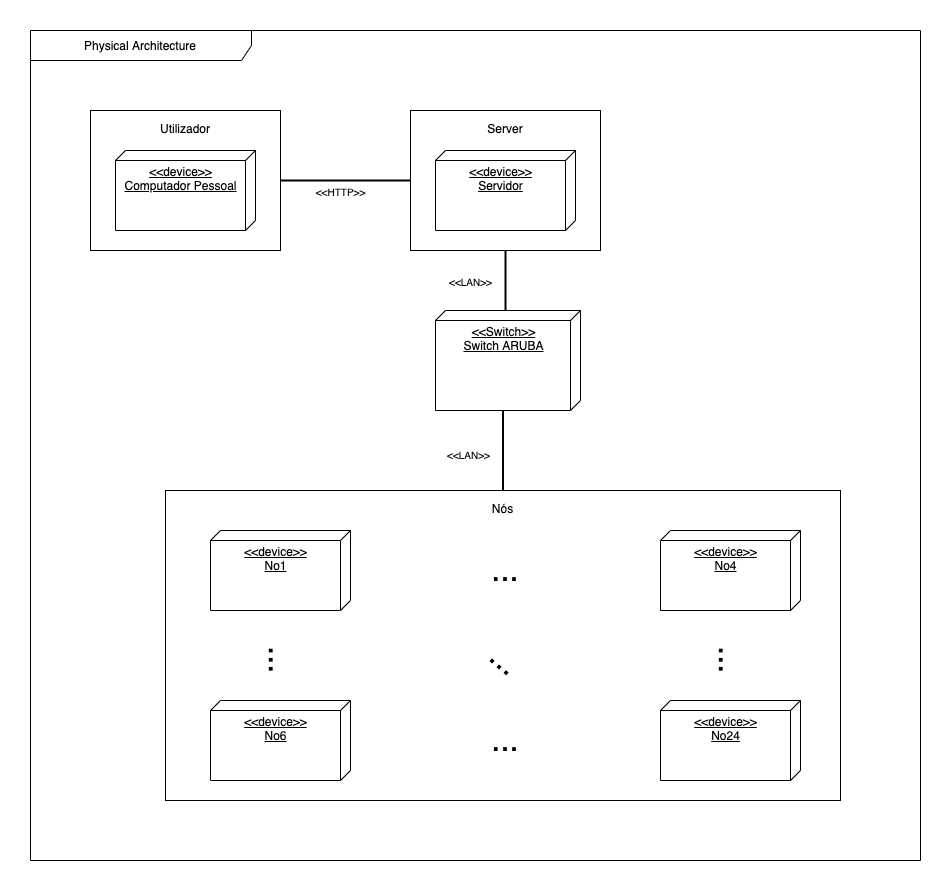
\includegraphics[height=0.68\textheight, width=1\textwidth]{images/physical_arch.png}
    \caption{Modelo Físico}
    \label{fig:fisico}
\end{figure}
É necessário que todas  as instâncias sejam acessíveis entre si, com exceção das bases de dados, onde, a Relacional só necessita estar acessível para o servidor principal Flask. O SQLite só necessita estar acessível para o servidor Django. É de realçar que o Switch Aruba teve que ser substituído devido aos impactos causados pelo Covid-19.

\subsection{Modelo Tecnológico}
O modelo tecnológico fornece uma vista sobre as tecnologias utilizadas pelo sistema. A figura seguinte demonstra como estas se relacionam entre si.

\begin{figure}[!ht]
    \centering
    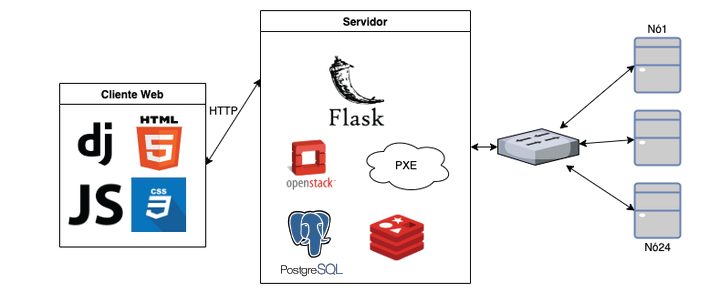
\includegraphics[height=0.3\textheight]{images/tecno.png}
    \caption{Modelo Tecnológico}
    \label{fig:tecno}
\end{figure}
\hfill\break
No lado do frontend, foi utilizada a framework Django que funciona sob a linguagem Python juntamente com HTML, JavaScript e CSS o que nos permitiu o desenvolvimento de uma plataforma web intuitiva e responsiva.\newline
No que toca ao armazenamento de dados, este é feito do lado do servidor e através do PostgreSQL - projeto open-source baseado em MySQL. \newline
Todas as ferramentas visíveis na imagem foram apresentadas e discutidas no capítulo 2. No que toca à sua implementação, razão de utilidade e a forma como interagem umas com as outras, no caso particular do projeto, serão discutidas abaixo.
\newpage
\hfill\break
%!TEX root = ../Report.tex
\chapter{Conclusão e Trabalho Futuro}
Morbi pharetra ligula integer mollis mi nec neque ultrices vitae volutpat leo ullamcorper. In at tellus magna. Curabitur quis posuere purus. Cum sociis natoque penatibus et magnis dis parturient montes, nascetur ridiculus mus. Suspendisse tristique placerat feugiat. Aliquam vitae est at enim auctor ultrices eleifend a urna. Donec non tincidunt felis. Maecenas at suscipit orci.


\appendix
%!TEX root = ../Report.tex

\chapter{Acrónimos}
\begin{acronym}[AMazING]
\acro{LEI}{Licenciatura em Engenharia Informática} 
\acro{UA}{Universidade de Aveiro} 
\acro{RDBMS}{Relational Database Management System} 
\acro{SQL}{Structured Query Language} 
\acro{HTML}{Hyper Text Markup Language} 
\acro{CSS}{Cascading Style Sheet} 
\acro{WWW}{World Wide Web}
\acro{UI}{User Interface}
\acro{CaU}{Casos de Uso}
\acro{REST}{Representational State Transfer}
\acro{API}{Application Programming Interface}
\acro{IT}{Instituto de Telecomunicações}
\acro{VM}{Máquina Virtual}
\acro{IaaS}{Infrastructure as a service (Infraestrutura como Serviço)}
\acro{GUI}{Graphic User Interface (Interface Gráfica do Utilizador)}
\acro{POE}{Power over Ethernet}
\acro{JWT}{Json Web Token}
\end{acronym}
%%!TEX root = ../Report.tex

%==============================================================================================================================================


\backmatter
\printbibliography[title=Referências]

\end{document}
